\PassOptionsToPackage{usenames}{color}
\documentclass[11pt,a4paper]{article}

\usepackage{relsize} % relative font sizes (e.g. \smaller). must precede ACL style
\usepackage{style/acl2015}
\usepackage[colorlinks=true,linkcolor=black,citecolor=black,filecolor=black,urlcolor=black]{hyperref}
\usepackage{natbib}

%\usepackage{times}
%\usepackage{latexsym}

\usepackage{microtype}

\usepackage[boxed]{algorithm2e}
\renewcommand\AlCapFnt{\small}
\usepackage[small,bf,skip=5pt]{caption}
\usepackage{sidecap} % side captions
\usepackage{rotating}	% sideways
% \usepackage[pdftex]{graphicx}

% Italicize subparagraph headings
\usepackage{titlesec}
\titleformat*{\subparagraph}{\itshape}
\titlespacing{\subparagraph}{%
  1em}{%              left margin
  0pt}{% space before (vertical)
  1em}%               space after (horizontal)

% Numbered Examples and lists
\usepackage{lingmacros}
\newcommand{\exref}[1]{(\ref{#1})} % numbered example

\usepackage[shortlabels]{enumitem} % customizable lists
\setitemize{noitemsep,topsep=0em,leftmargin=*}
\setenumerate{noitemsep,leftmargin=0em,itemindent=13pt,topsep=0em}

\usepackage{xspace}
\usepackage{xparse} % for fancy custom macros (\NewDocumentEnvironment, etc.)

\newcommand{\indicator}[1]{\boldsymbol{1}\{#1\}}


\usepackage{textcomp}
% \usepackage{arabtex} % must go after xparse, if xparse is used!
%\usepackage{utf8}
% \setcode{utf8} % use UTF-8 Arabic
% \newcommand{\Ar}[1]{\RL{\novocalize #1}} % Arabic text

\usepackage{framed}

\usepackage{listings}

\lstset{
  basicstyle=\itshape,
  xleftmargin=3em,
  aboveskip=0pt,
  belowskip=-3pt, %-.5\baselineskip, % correct for extra paragraph break inserted after listing
  literate={->}{$\rightarrow$}{2}
           {α}{$\alpha$}{1}
           {δ}{$\delta$}{1}
           {(}{$($}{1}
           {)}{$)$}{1}
           {[}{$[$}{1}
           {]}{$]$}{1}
           {|}{$|$}{1}
           {+}{\ensuremath{^+}}{1}
           {*}{\ensuremath{^*}}{1}
}

\usepackage{amssymb}	%amsfonts,eucal,amsbsy,amsthm,amsopn
\usepackage{amsmath}

\usepackage{mathptmx}	% txfonts
\usepackage[scaled=.8]{beramono}
\usepackage[scaled=.85]{helvet}
\usepackage[T1]{fontenc}
\usepackage[utf8x]{inputenc}

\usepackage{MnSymbol}	% must be after mathptmx

\usepackage{latexsym}





% Tables
\usepackage{array}
\usepackage{multirow}
\usepackage{booktabs} % pretty tables
\usepackage{multicol}
\usepackage{footnote}
\newcolumntype{H}{>{\setbox0=\hbox\bgroup}c<{\egroup}@{}} % hidden column


\usepackage{url}
\usepackage[usenames]{color}
\usepackage{xcolor}

% colored frame box
\newcommand{\cfbox}[2]{%
    \colorlet{currentcolor}{.}%
    {\color{#1}%
    \fbox{\color{currentcolor}#2}}%
}

\usepackage[normalem]{ulem} % \uline
\usepackage{colortbl}
\usepackage{graphicx}
\usepackage{subcaption}
%\usepackage{tikz-dependency}
\usepackage{tikz}
%\usepackage{tree-dvips}
\usetikzlibrary{arrows,positioning,calc} 

\DeclareMathOperator*{\argmax}{arg\,max}
\DeclareMathOperator*{\argmin}{arg\,min}
%\setlength\titlebox{6.5cm}    % Expanding the titlebox
\setlength\titlebox{5.5cm}    % Expanding the titlebox

\usepackage{nameref}
\usepackage{cleveref}

% use \S for all references to all kinds of sections, and \P to paragraphs
% (sadly, we cannot use the simpler \crefname{} macro because it would insert a space after the symbol)
\crefformat{part}{\S#2#1#3}
\crefformat{chapter}{\S#2#1#3}
\crefformat{section}{\S#2#1#3}
\crefformat{subsection}{\S#2#1#3}
\crefformat{subsubsection}{\S#2#1#3}
\crefformat{paragraph}{\P#2#1#3}
\crefformat{subparagraph}{\P#2#1#3}
%\crefmultiformat{part}{\S#2#1#3}{ and~\S#2#1#3}{, \S#2#1#3}{, and~\S#2#1#3}
%\crefmultiformat{chapter}{\S#2#1#3}{ and~\S#2#1#3}{, \S#2#1#3}{, and~\S#2#1#3}
\crefmultiformat{section}{\S#2#1#3}{ and~\S#2#1#3}{, \S#2#1#3}{, and~\S#2#1#3}
\crefmultiformat{subsection}{\S#2#1#3}{ and~\S#2#1#3}{, \S#2#1#3}{, and~\S#2#1#3}
\crefmultiformat{subsubsection}{\S#2#1#3}{ and~\S#2#1#3}{, \S#2#1#3}{, and~\S#2#1#3}
\crefmultiformat{paragraph}{\P\P#2#1#3}{ and~#2#1#3}{, #2#1#3}{, and~#2#1#3}
\crefmultiformat{subparagraph}{\P\P#2#1#3}{ and~#2#1#3}{, #2#1#3}{, and~#2#1#3}
%\crefrangeformat{part}{\mbox{\S\S#3#1#4--#5#2#6}}
%\crefrangeformat{chapter}{\mbox{\S\S#3#1#4--#5#2#6}}
\crefrangeformat{section}{\mbox{\S\S#3#1#4--#5#2#6}}
\crefrangeformat{subsection}{\mbox{\S\S#3#1#4--#5#2#6}}
\crefrangeformat{subsubsection}{\mbox{\S\S#3#1#4--#5#2#6}}
\crefrangeformat{paragraph}{\mbox{\P\P#3#1#4--#5#2#6}}
\crefrangeformat{subparagraph}{\mbox{\P\P#3#1#4--#5#2#6}}
% for \label[appsec]{...}
\crefname{part}{Part}{Parts}
\Crefname{part}{Part}{Parts}
\crefname{chapter}{ch.}{ch.}
\Crefname{chapter}{Ch.}{Ch.}
\crefname{figure}{figure}{figures}
\crefname{appsec}{appendix}{appendices}
\Crefname{appsec}{Appendix}{Appendices}
\crefname{algocf}{algorithm}{algorithms}
\Crefname{algocf}{Algorithm}{Algorithms}
\crefname{enums,enumsi}{example}{examples}
\Crefname{enums,enumsi}{Example}{Examples}
\crefname{}{example}{examples} % lingmacros \toplabel has no internal name for the kind of label
\Crefname{}{Example}{Examples}
\crefformat{enums}{(#2#1#3)}
\crefformat{enumsi}{(#2#1#3)}
\crefformat{}{(#2#1#3)}
\crefrangeformat{enums}{\mbox{(#3#1#4--#5#2#6)}}
\crefrangeformat{enumsi}{\mbox{(#3#1#4--#5#2#6)}}

\ifx\creflastconjunction\undefined%
\newcommand{\creflastconjunction}{, and\nobreakspace} % Oxford comma for lists
\else%
\renewcommand{\creflastconjunction}{, and\nobreakspace} % Oxford comma for lists
\fi%

\newcommand*{\Fullref}[1]{\hyperref[{#1}]{\Cref*{#1}: \nameref*{#1}}}
\newcommand*{\fullref}[1]{\hyperref[{#1}]{\cref*{#1}: \nameref{#1}}}
\newcommand{\fnref}[1]{fn.~\ref{#1}} % don't use \cref{} due to bug in (now out-of-date) cleveref package w.r.t. footnotes
\newcommand{\Fnref}[1]{Fn.~\ref{#1}}


\newcommand{\backtick}[0]{\textasciigrave}


\NewDocumentEnvironment{itmize}{}{\begin{itemize}[noitemsep]}{\end{itemize}}
\NewDocumentEnvironment{enumrate}{}{\begin{enumerate}[noitemsep]}{\end{enumerate}}
\let\Item\item
\renewcommand\enddescription{\endlist\global\let\item\Item}
\NewDocumentEnvironment{describe}{}{\renewcommand\item[1][]{\Item \textbf{##1:} }\begin{itemize}}{\end{itemize}}
\NewDocumentEnvironment{edescribe}{}{\renewcommand\item[1][]{\Item \textbf{##1:} }\begin{enumerate}}{\end{enumerate}}


% Author comments
\usepackage{color}
\newcommand\bmmax{0} % magic to avoid 'too many math alphabets' error
\usepackage{bm}
\definecolor{orange}{rgb}{1,0.5,0}
\definecolor{mdgreen}{rgb}{0,0.6,0}
\definecolor{mdblue}{rgb}{0,0,0.7}
\definecolor{dkblue}{rgb}{0,0,0.5}
\definecolor{dkgray}{rgb}{0.3,0.3,0.3}
\definecolor{slate}{rgb}{0.25,0.25,0.4}
\definecolor{gray}{rgb}{0.5,0.5,0.5}
\definecolor{ltgray}{rgb}{0.7,0.7,0.7}
\definecolor{purple}{rgb}{0.7,0,1.0}
\definecolor{lavender}{rgb}{0.65,0.55,1.0}

% Settings for algorithm listings
% \lstset{
%   language=Python,
%   upquote=true,
%   showstringspaces=false,
%   formfeed=\newpage,
%   tabsize=1,
%   commentstyle=\itshape\color{lavender},
%   basicstyle=\small\smaller\ttfamily,
%   morekeywords={lambda},
%   emph={upward,downward,tc},
%   emphstyle=\underbar,
%   aboveskip=0cm,
%   belowskip=-.5cm
% }
%\renewcommand{\lstlistingname}{Algorithm}


\newcommand{\ensuretext}[1]{#1}
\newcommand{\cjdmarker}{\ensuretext{\textcolor{green}{\ensuremath{^{\textsc{CJ}}_{\textsc{D}}}}}}
\newcommand{\nssmarker}{\ensuretext{\textcolor{magenta}{\ensuremath{^{\textsc{NS}}_{\textsc{S}}}}}}
\newcommand{\mkmarker}{\ensuretext{\textcolor{red}{\ensuremath{^{\textsc{M}}_{\textsc{K}}}}}}
\newcommand{\stmarker}{\ensuretext{\textcolor{blue}{\ensuremath{^{\textsc{S}}_{\textsc{T}}}}}}
\newcommand{\jbmarker}{\ensuretext{\textcolor{orange}{\ensuremath{^{\textsc{J}}_{\textsc{B}}}}}}
\newcommand{\dbmarker}{\ensuretext{\textcolor{purple}{\ensuremath{^{\textsc{D}}_{\textsc{B}}}}}}
\newcommand{\arkcomment}[3]{\ensuretext{\textcolor{#3}{[#1 #2]}}}
%\newcommand{\arkcomment}[3]{}
\newcommand{\cjd}[1]{\arkcomment{\cjdmarker}{#1}{green}}
\newcommand{\nss}[1]{\arkcomment{\nssmarker}{#1}{magenta}}
\newcommand{\mk}[1]{\arkcomment{\mkmarker}{#1}{red}}
\newcommand{\st}[1]{\arkcomment{\stmarker}{#1}{blue}}
\newcommand{\jb}[1]{\arkcomment{\jbmarker}{#1}{orange}}
\newcommand{\db}[1]{\arkcomment{\dbmarker}{#1}{purple}}
\newcommand{\wts}{\mathbf{w}}
\newcommand{\g}{\mathbf{g}}
\newcommand{\f}{\mathbf{f}}
\newcommand{\x}{\mathbf{x}}
\newcommand{\y}{\mathbf{y}}
\newcommand{\overbar}[1]{\mkern 1.5mu\overline{\mkern-1.5mu#1\mkern-1.5mu}\mkern 1.5mu} % \bar is too narrow in math
\newcommand{\cost}{c}

\newcommand{\term}[1]{\textbf{#1}} % term being defined

\newcommand{\citeposs}[2][]{\citeauthor{#2}'s (\citeyear[#1]{#2})}
\newcommand{\Citeposs}[2][]{\Citeauthor{#2}'s (\citeyear[#1]{#2})}

% Space savers
% From http://www.eng.cam.ac.uk/help/tpl/textprocessing/squeeze.html
\addtolength{\dbltextfloatsep}{-.5cm} % space between last top float or first bottom float and the text.
%\addtolength{\intextsep}{-1cm} % space left on top and bottom of an in-text float.
\addtolength{\abovedisplayskip}{-1cm} % space before maths
\addtolength{\belowdisplayskip}{-1cm} % space after maths
%\addtolength{\topsep}{-.5cm} %space between first item and preceding paragraph
%\setlength{\belowcaptionskip}{-.3cm}
\setlength{\intextsep}{0pt plus 2pt}   % default value 12pt plus 2pt minus 2pt


% customize \paragraph spacing
\makeatletter
\renewcommand{\paragraph}{%
  \@startsection{paragraph}{4}%
  {\z@}{.2ex \@plus 1ex \@minus .2ex}{-1em}%
  {\normalfont\normalsize\bfseries}%
}
\makeatother



% Special macros
\newcommand{\lbl}[1]{\textsc{#1}} % class label
\newcommand{\sst}[1]{\lbl{#1}} % supersense tag label
\newcommand{\nsst}[1]{\sst{n:#1}} % noun supersense tag label
\newcommand{\vsst}[1]{\sst{v:#1}} % verb supersense tag label


\newcommand{\tg}[1]{\texttt{#1}}	% supersense tag name
\newcommand{\gfl}[1]{%\renewcommand\texttildelow{{\lower.74ex\hbox{\texttt{\char`\~}}}} % http://latex.knobs-dials.com/
\mbox{\textsmaller{\texttt{#1}}}}	% supersense tag symbol
 \newcommand{\tagdef}[1]{#1\hfill} % tag definition
\newcommand{\tagt}[2]{\ensuremath{\underset{\textrm{\textlarger{\tg{#2}}}\strut}{\w{#1}\rule[-.3\baselineskip]{0pt}{0pt}}}} % tag text (a word or phrase) with an SST. (second arg is the tag)
\newcommand{\glosst}[2]{\ensuremath{\underset{\textrm{#2}}{\textrm{#1}}}} % gloss text (a word or phrase) (second arg is the gloss)
\newcommand{\AnnA}[0]{\mbox{\textbf{Ann-A}}} % annotator A
\newcommand{\AnnB}[0]{\mbox{\textbf{Ann-B}}} % annotator B
\newcommand{\sys}[1]{\mbox{\textbf{#1}}}   % name of a system (one of our experimental conditions)
\newcommand{\dataset}[1]{\mbox{\textsc{#1}}}	% one of the datasets in our experiments
\newcommand{\datasplit}[1]{\mbox{\textbf{#1}}}	% portion one of the datasets in our experiments

\newcommand{\fnf}[1]{\textsc{\textsf{#1}}} % FrameNet frame
\newcommand{\fnr}[1]{\textbf{\textsf{#1}}} % FrameNet role (frame element name)
\newcommand{\fnlu}[1]{\textsf{#1}} % FrameNet lexical unit (predicate)

%\newcommand{\lex}[1]{\textsmaller{\textsf{\textcolor{slate}{\textbf{#1}}}}}	% example lexical item
\newcommand{\lex}[1]{\textit{#1}} % lexical item/lexical example
\newcommand{\pex}[1]{\textit{#1}} % phrasal example - don't index by default

%\newcommand{\w}[1]{\textit{#1}}	% word
\newcommand{\gap}[0]{\ \ } % space around gap contents
\newcommand{\tat}[0]{\textasciitilde}

\newcommand{\shortlong}[2]{#1} % short vs. long version of the paper
\newcommand{\confversion}[1]{#1}
\newcommand{\srsversion}[1]{}
\newcommand{\finalversion}[1]{}
%\newcommand{\finalversion}[1]{}
\newcommand{\shortversion}[1]{#1}
\newcommand{\considercutting}[1]{#1}
\newcommand{\longversion}[1]{} % ...if only there were more space...
\newcommand{\subversion}[1]{#1} % for the submission version only
\newcommand{\draftnotice}[1]{} % for the draft version only
%\newcommand{\subversion}[1]{}

%%%%%%%%%% HYPHENATION

\hyphenation{WordNet}
\hyphenation{WordNets}
\hyphenation{FrameNet}
\hyphenation{SemCor}
\hyphenation{SemEval}
\hyphenation{ParsedSemCor}
\hyphenation{VerbNet}
\hyphenation{PennConverter}
\hyphenation{an-aly-sis}
\hyphenation{an-aly-ses}
\hyphenation{base-line}
\hyphenation{comb-over}
\hyphenation{de-ve-lop-ed}
\hyphenation{news-text}
\hyphenation{nomi-nal}
\hyphenation{per-cept}
\hyphenation{per-cepts}
\hyphenation{post-edit-ing}
\hyphenation{shriv-eled}
\hyphenation{Huddle-ston}

\title{\nss{provisional title:}Leveraging Additional Resources for Frame-Semantic Role Labeling}

% Nathan Schneider, Shay B. Cohen, and Noah A. Smith 
% \author{Nathan Schneider \quad Emily Danchik \quad Chris Dyer \quad Noah A. Smith \\
% 	    School of Computer Science\\
% 	    Carnegie Mellon University\\
% 	    Pittsburgh, PA 15213, USA\\
% 	    {\tt \{nschneid,emilydan,cdyer,nasmith\}@cs.cmu.edu}}

% \author{Author 1\\
% 	    XYZ Company\\
% 	    111 Anywhere Street\\
% 	    Mytown, NY 10000, USA\\
% 	    {\tt author1@xyz.org}
% 	  \And
% 	Author 2\\
%   	ABC University\\
%   	900 Main Street\\
%   	Ourcity, PQ, Canada A1A 1T2\\
%   {\tt author2@abc.ca}}

\date{}

\begin{document}
\maketitle
\begin{abstract}
The high cost of semantic structure annotation is a major obstacle 
to automating semantic analysis with broad coverage.
The fully annotated datasets that exist are often small, 
hindering the robustness of models trained on them.
However, low-resource tasks may benefit from exploiting \emph{partially} annotated data, 
as well as data with \emph{different} (but related) forms of annotation,
for additional training data or features.
This paper considers the argument identification and classification subtask 
of frame-semantic parsing, which to date has relied exclusively 
upon full-text annotations in the FrameNet resource.\nss{is this true? I think Dipanjan used exemplars for the latent variable frame ID model, but he hasn't used them at all for arg ID, right?}
We augment supervised learning with additional 
``indirect'' training data and features 
so as to leverage additional resources internal and external to FrameNet (e.g., PropBank). 
\nss{result}
\end{abstract}

\section{Introduction}

\nss{sparseness is a challenge for many computational semantics tasks}

Frame-semantic parsing \citep{das-14} is a case in point.
This is the task of automating the rich linguistic structure analyses 
of the FrameNet lexicon and corpus \citep{baker-98}.\footnote{\url{http://framenet.icsi.berkeley.edu/}}
FrameNet represents kinds of events, scenarios, and relationships 
with an inventory of \textbf{frames} (\nss{examples}). 
Each frame is associated with lexical \textbf{predicates} (verbs, nouns, adjectives, and adverbs) capable of 
evoking the scenario, and a set of \textbf{roles} (or \textbf{frame elements}) 
called to mind in order to understand the scenario. 
These roles may be implicit, 
but are frequently realized linguistically in the same sentence as the predicate.
Given a sentence, frame-semantic parsing is the task of mapping tokens in the sentences
to evoked frames, and for each evoked frame, finding and labeling its \textbf{argument} phrases 
with roles. 
An example appears in \cref{fig:harbor-fn}; it will be explained in detail in \cref{sec:ft}.

\begin{figure}
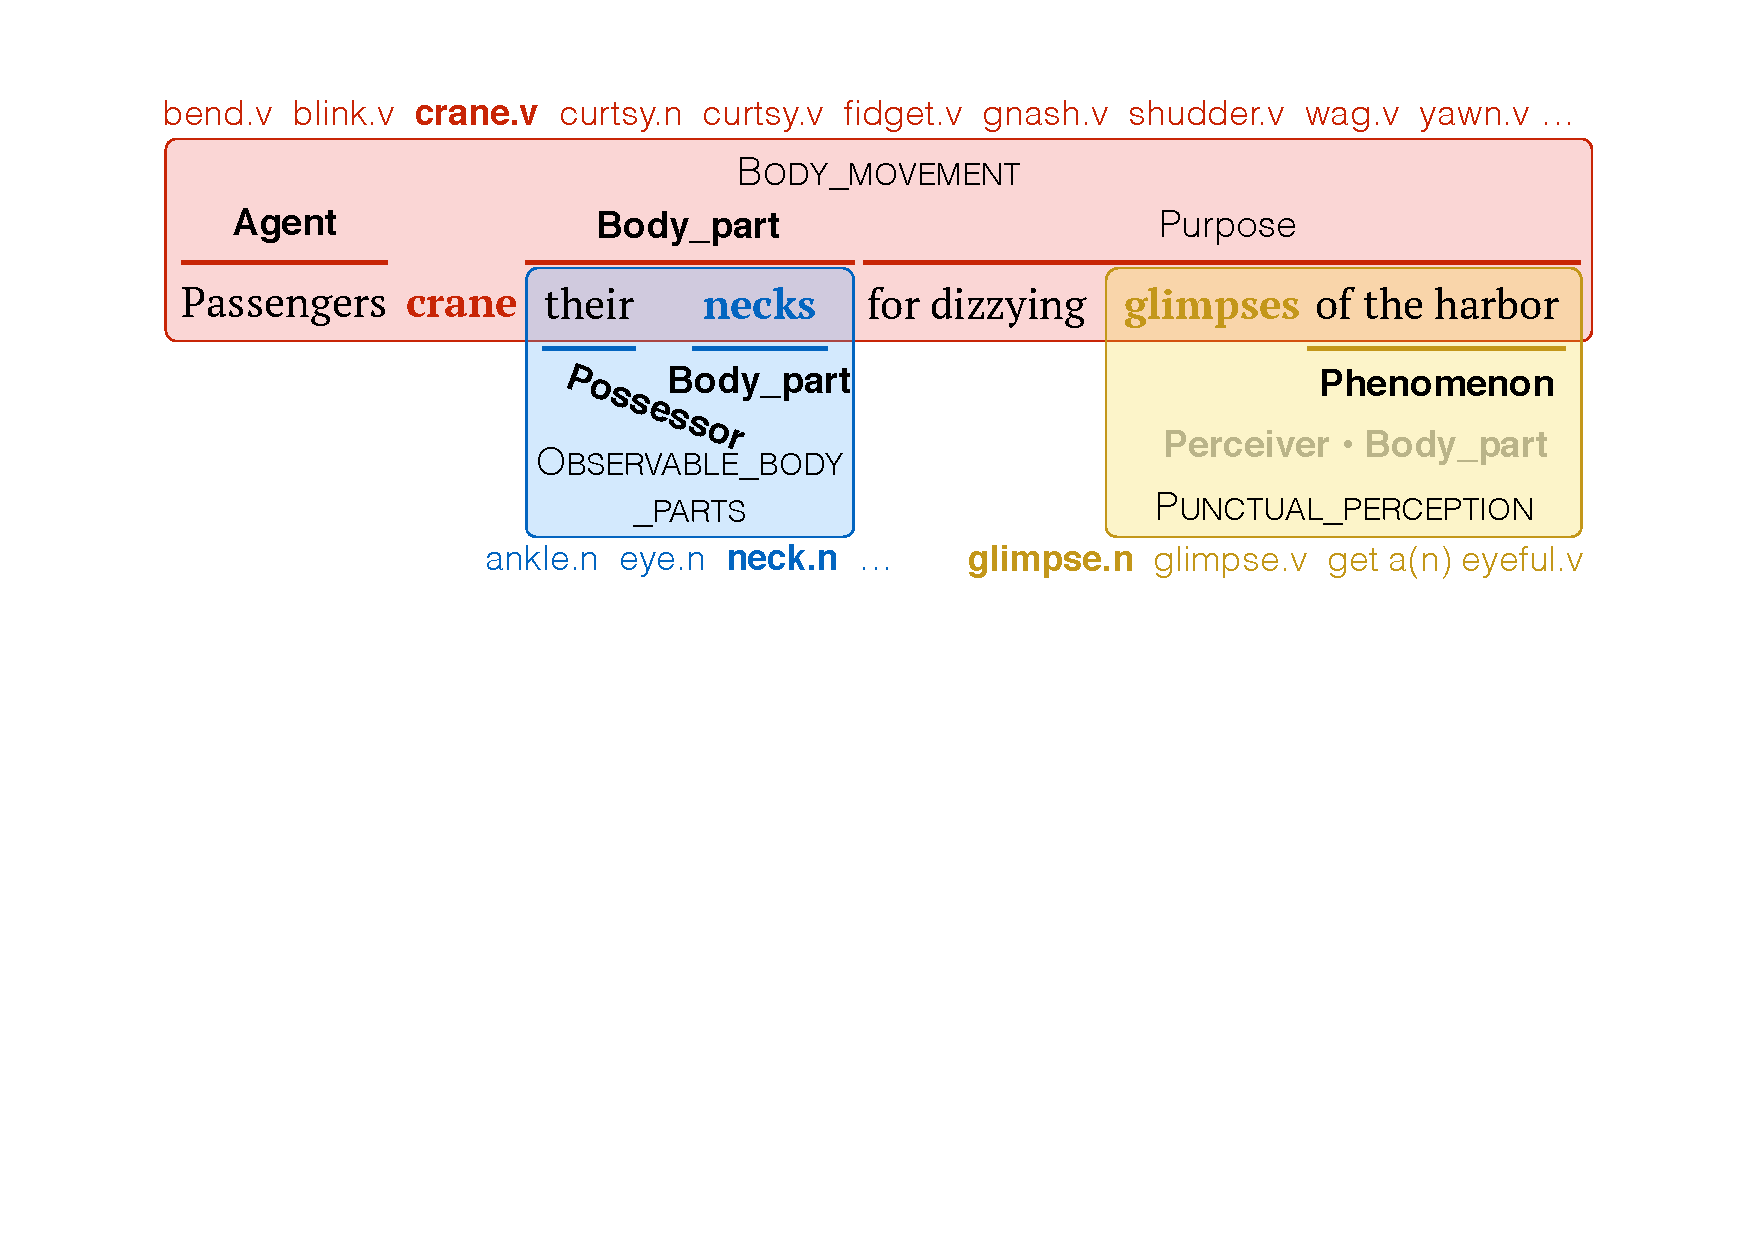
\includegraphics[width=\columnwidth]{harbor-fn.pdf}
\caption{Example sentence from FrameNet full-text annotation. 
3~frames and their arguments are shown: 
\fnf{Body\_movement} is evoked by \textit{crane},
\fnf{Observable\_body\_parts} by \textit{necks}, 
and \fnf{Punctual\_perception} by \textit{glimpse}.
(Further, \textit{harbor} is annotated as evoking the \fnf{Locale\_by\_use} frame 
and doubles as its sole argument.) 
Horizontal lines representing argument spans 
are labeled with role names.}
\label{fig:harbor-fn}
\end{figure}

FrameNet~1.5 defines a structured hierarchy of over 1,000 frames associated with \nss{\#}~English lexical predicates, 
and also provides annotations for \nss{\# targets annotated total} attestations 
of these frames/predicates in corpora, annotated in context with their arguments. 
In FrameNet~1.5, a rather small number of sentences---\nss{\#}, comprising \nss{\#} words---% 
are provided with \textbf{full-text} annotations, i.e.~the sentence 
has been analyzed for all available frames. 
But a full \nss{\#}\% of sentences in FrameNet---the lexicographic \textbf{exemplars}---are annotated for only one frame per sentence, 
and have thus far not been exploited successfully for frame-semantic parsing.
Here, we seek to leverage these exemplar sentences 
as well as the (type-level) hierarchical structure of the FrameNet lexicon. 

\begin{figure}
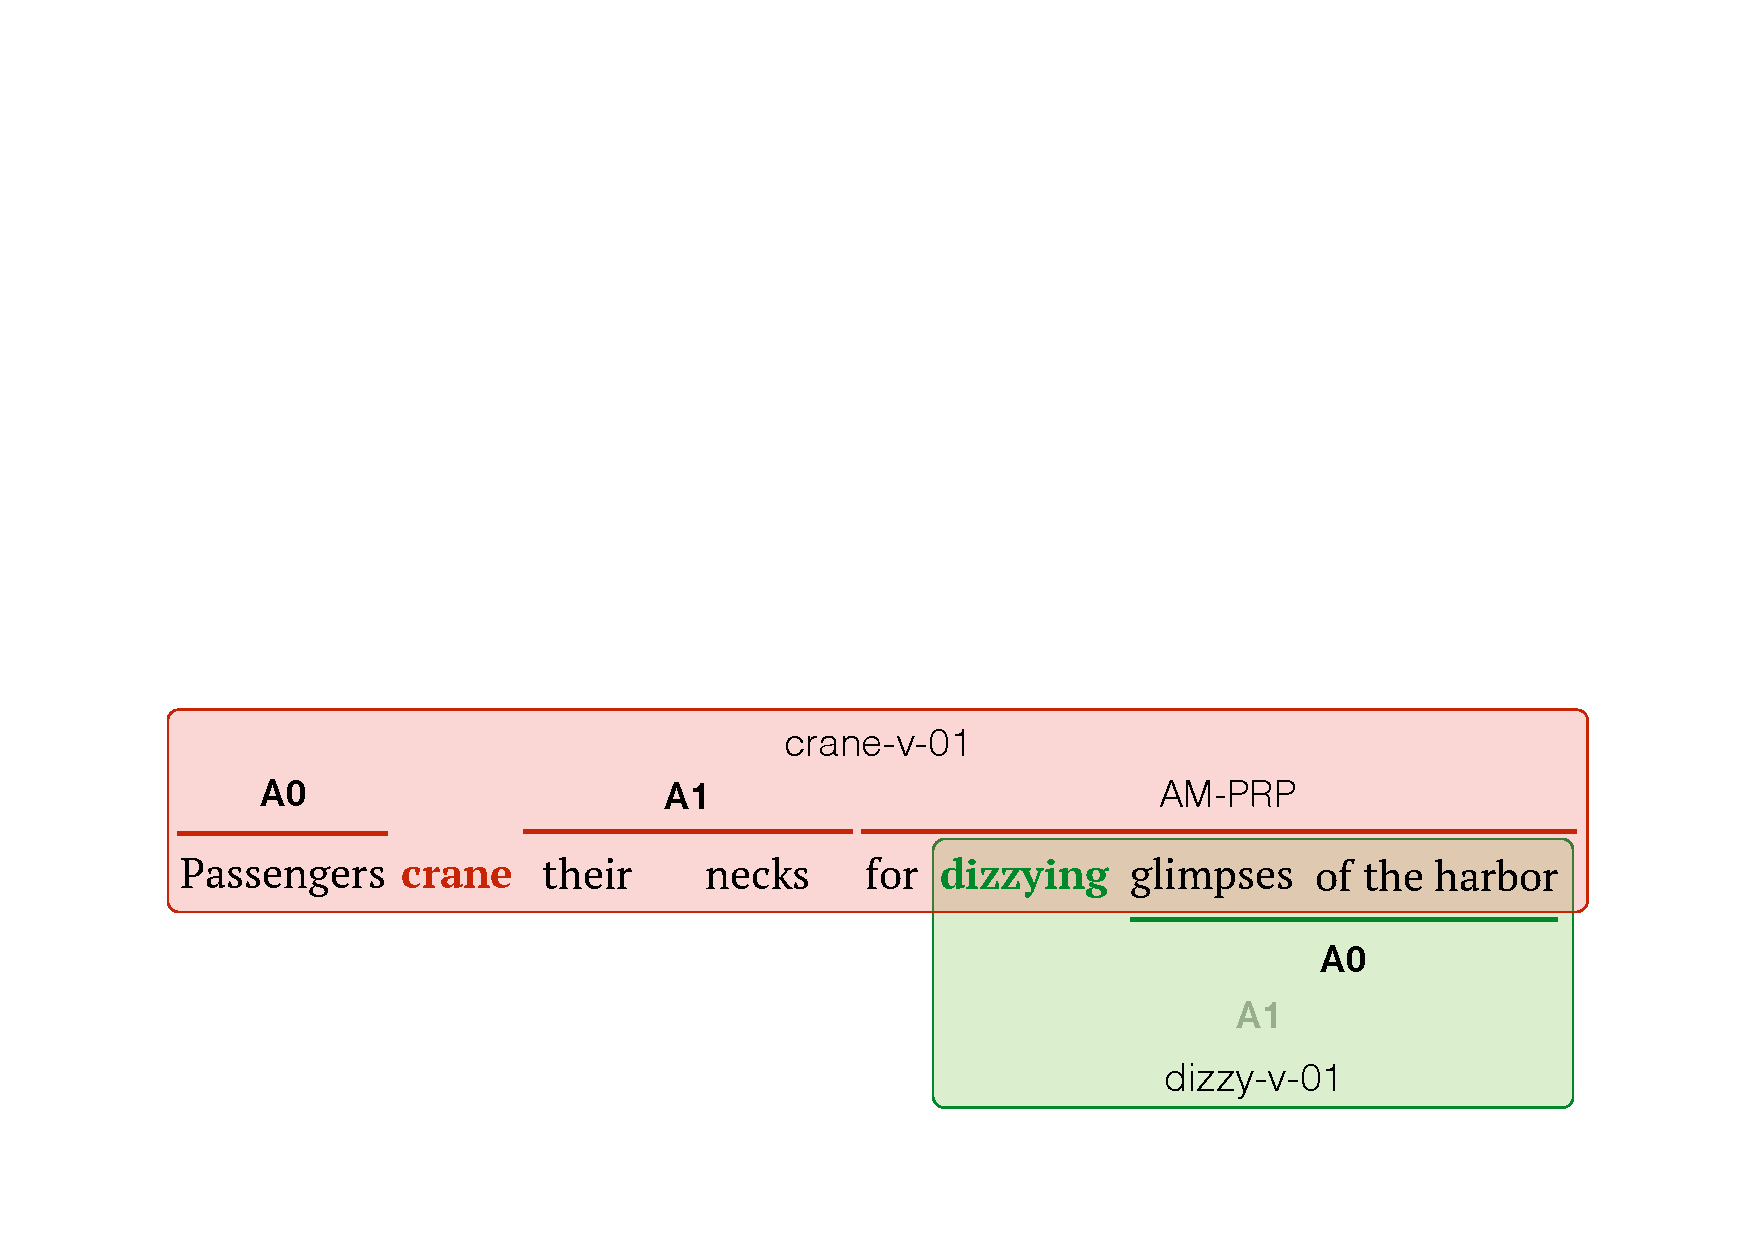
\includegraphics[width=\columnwidth]{harbor-pb.pdf}
\caption{Ideal PropBank annotations for verbs. Though PB uses lexical frames rather than deep frames,
there are clear similarities to the FrameNet annotations in \cref{fig:harbor-fn}.}
\label{fig:harbor-pb}
\end{figure}

In this paper, we address the \textbf{argument identification} 
subtask of finding and labeling arguments 
given a predicate in context and the frame it evokes.
This is a form of semantic role labeling (SRL).
\st{cite Gildea, Roth, Toutanova, etc.}
Notably, another resource, \textbf{PropBank} \citep{propbank}, has been widely used for SRL \citep{palmer-10}. 
PropBank annotations capture shallower lexical frames and arguments; 
additionally, PropBank provides \nss{millions?} of words of fully annotated English sentences
(annotation is much less expensive, but also potentially less valuable, because of the shallower representation).
Despite a number of differences in the representations and annotation conventions, 
for many predicates FrameNet and PropBank are really quite similar: 
\cref{fig:harbor-fn} and \cref{fig:harbor-pb} show this for the verb \textit{crane}.
To get the best of both worlds, we aim to tap into PropBank's vast resources 
as indirect token-level supervision for FrameNet-style analysis. 
We hypothesize that PropBank analyses can serve as a weak signal for the FrameNet SRL task, 
either by heuristically transforming PropBank annotations into FrameNet annotations 
to augment the training data, or by preprocessing sentences with a PropBank SRL system to obtain new features 
for FrameNet argument identification.

Our experiments expand the \emph{training data} and/or the \emph{feature space}
of supervised argument identification
in order to integrate evidence from all of these sources 
into SEMAFOR \citep{das-14}, the leading open-source frame-semantic parser for English.\footnote{\url{http://www.ark.cs.cmu.edu/SEMAFOR/}} 
The results show that some of these sources of evidence succeed 
at boosting argument identification performance.\nss{SOTA (without constraints)?}


\section{Resources}

\nss{incl. data analysis of differences from full-text}

\nss{w/in each mention: genre/overall vocabulary; coverage and distributions of predicates, FE labels; oracle coverage of FT test}

\subsection{The FrameNet Lexicon}\label{sec:lex}

Each frame in the Berkeley FrameNet lexicon is intended to represent a gestalt scene. 
The frame definition includes: a descriptive name; 
a set of \textbf{core roles} representing participants and props that are crucial 
to understanding the scene; a set of \textbf{non-core roles} such as circumstantial 
information (time, place, manner, purpose, etc.); 
an English textual description of the scene and how its roles relate to one another;
and a set of English predicates that can evoke the scene.
For example, the \fnf{Body\_movement} frame has \fnr{Agent} and \fnr{Body\_part} as its core roles; 
the frame description states,
``This frame contains words for motions or actions an \fnr{Agent} performs using some part of his/her body.''
Lexical entries in this frame include verbs such as \fnlu{bend}, \fnlu{blink}, \fnlu{crane}, and \fnlu{curtsy}, 
plus the noun use of \fnlu{curtsy}.

\nss{hierarchy. which relations do we care about---anything besides Inheritance?}

\subsection{Full-text Annotations}\label{sec:ft}

Contemporary frame-semantic parsers are trained and evaluated on the \textbf{full-text (FT)}\footnote{Though these 
were \emph{annotated} and the document level, and train/dev/test splits are by document, the frame-semantic parsing 
is currently restricted to the sentence level.} portion 
of the FrameNet corpus. This consists of documents for which annotators made an effort 
to assign frames and arguments to as many words as possible. 
\Cref{fig:harbor-fn} gives an example sentence from the FT portion of the corpus. 
It has 4~frame annotations. \fnf{Body\_movement}, as described in the previous section, 
is evoked by \textit{crane}, and 3~of its roles are filled by overt arguments: 
the 2~core roles (\fnr{Agent}, \fnr{Body\_part}) happen to be filled by noun phrases 
(\textit{passengers}, \textit{their necks}), while the non-core role \fnr{Purpose} is filled by a 
prepositional phrase adjunct (\textit{for dizzying glimpses of the harbor}).
The frame defines 19~additional non-core roles, none of which have an argument in the example.
In frame semantics, non-core roles are considered to be \emph{conceptually} optional; 
core roles may or may not be \emph{syntactically} optional, but if not locally specified they are 
expected to be available from context, or else implicit.
For example, \fnf{Punctual\_perception}---evoked in this case by \textit{glimpses}---is annotated 
as missing 2~of its core roles. A human listener would resolve the identity of the \fnr{Perceiver} 
from the wider context and the \fnr{Body\_part} from world knowledge. 

In some cases, FT annotation involved creating a new frame or adding a new lexical unit to an existing frame. 
In other cases, words that in principle should be considered to evoke a frame were left unannotated 
because they did not match any existing lexical units. 
This was the case for \textit{passengers} and \textit{dizzying} in \cref{fig:harbor-fn}.

Genres, sizes

Annotation density: (proportion of tokens evoking a frame. breakdown by POS?)

\subsection{Exemplars}\label{sec:exemplars}

\nss{how different from FT}

\subsection{PropBank}\label{sec:pb}

\nss{how different from FN}

\subsection{SemLink}\label{sec:semlink}

\nss{limitations!}

\subsection{Illinois SRL system}



\section{Learning from multiple domains and representations}



We experiment with several techniques for modifying the model-fitting portion of 
the argument identification model's local learning objective 
(training data, features). All of our experiments use the same form of regularization, 
condition on the same frame predictions\nss{not oracle, right? these are SEMAFOR's current frame ID model, so not state of the art?} 
and syntactic preprocessing\nss{does this match Dipanjan's latest experiments?}, 
and use beam search with \nss{hyperparam value} for joint decoding of arguments.\footnote{\nss{recent work has improved upon global decoding techniques; we expect such improvements to be complementary to the gains due to the local model reported here}}

\nss{Domain adaptation/multitask learning techniques}

\subsection{Augmenting the Training Data}

\subsection{Frustratingly Easy}

\subsection{2-stage}

\subsection{Type-level hierarchy features}
\mk{Types of relations and the number of relations of each type used: Inheritance and Subframe. How many types of relations?}

Frames in FrameNet are connected to each other by relations such as inheritance, temporal ordering, causality. 
For instance, the frame \fnf{Robbery} inherits from the more abstract frame \textit{Committing\_crime}, the 
frame \fnf{Fall\_asleep} is preceeded by the frame \fnf{Being\_awake}. The roles of related frames have 
also been mapped to indicate the correspondence between them: \fnf{Robbery}.\fnr{Perpetrator} is mapped to 
\fnf{Committing\_crime}.\fnr{Perpetrator} which in turn maps to \fnf{Misdeed}.\fnr{Wrongdoer}. Frames and roles that are far
apart in this hierarchy are less related than say neighbours.
This hierarchy can be exploited to share information across related roles, thereby benefiting the roles 
that have few annotations \mk{say something about a greater variety of contexts is available for each role}. 
A simple mechanism to share information is via shared model parameters between related roles. Towards this, we define two types of
hierarchical features: (1) `siblings', where for every feature $f_i$ that fires for an argument $a$, we add a feature which is the conjunction: 
$(f_i \wedge \textrm{parent.frame} \wedge \textrm{parent.role} \wedge I_{hier})$ where parent.frame = parent(frame($a$)). 
$I_{hier}$ is an indicator to distinguish this feature from the regular conjunction features that use frame names and roles.
(2) `parents', where the addendum is the feature: $(f_i \wedge \textrm{frame} \wedge \textrm{frame.role} \wedge I_{hier})$.
We use only the `Inheritance' and 'Subframe' relations between the roles, of which there are 4138 and 589 respectively.


\section{Experiments}

\nss{tuning regularizer for all experiments}




\subsection{Baseline}

% In FrameNet parlance, a \term{target} is a contiguous span of tokens in a sentence that evokes a \term{frame}.
% Each frame has its own fixed set of possible role names, or \term{frame elements}, that can either be realized or not.
% If they are realized, the span of tokens filling the role are annotated.
% If not, the frame element is said to have a \term{null instantiation}\st{check my terminology}.
% \st{example?}
% The \term{argument identification} task is to automatically generate these frame element annotations, given a gold-standard target and its evoked frame.

Our baseline system is SEMAFOR \citep{das-14}.
SEMAFOR treats the argument identification task as a structured prediction problem.
It uses a linearly parametrized model that scores each candidate span given a frame element\st{this should probably be talked about earlier?}:
\begin{equation}
\text{score}_\mathbf{w}(y \mid x) = \mathbf{w}^\top \mathbf{f}(x, y)
\end{equation}
Automatic syntactic parses \st{from where? are we using the MST-stacked dep parses?} are used to narrow the set of candidate spans considered, and as input to feature extraction.

During training, each frame element is treated as an independent multiclass logistic regression instance, with the set of candidate spans (including the \textsc{NULL} span) as its output space.
But at test time, it chooses a joint assignment of all arguments that maximizes probability under the model, while satisfying the following constraints:
\begin{enumerate}
  \item an argument may be assigned to at most one span \st{theta criterion, Chomsky}, and
  \item spans of realized arguments must not overlap.
\end{enumerate}
Beam search, with a beam size of 100, is used to choose the maximum joint assignment with no overlapping arguments.
\nss{does beam search require normalizing to probabilities?}

We have made several modifications to SEMAFOR's training that do not affect performance, but do speed up experiments:

\begin{itemize}
  \item We use squared structured hinge loss (defined below) instead of multiclass logistic regression.
  Using hinge loss, there is no longer a need to calculate a partition function.
  Gradients, and hence parameters, are sparser than in logistic regression, allowing us to use a sparse vector implementation.
  \item We use the online optimization method AdaDelta \citep{zeiler-12} with minibatches\nss{minibatch size?}, instead of the batch method L-BFGS \citep{liu-89}.
  \item We use elastic net ($\ell_1 + \ell_2$) regularization. Adding $\ell_1$ also has the effect of keeping the parameter vector sparse.\nss{what hyperparameter(s)? are $\ell_1$ and $\ell_2$ tuned separately?}
\end{itemize}
We use these changes for all systems, including the baseline.
While performance is not significantly affected \mk{P/R/F numbers are in the table (see rows 1 and 2). Times: 12 hrs 9 mins for the earlier algorithm to converge. That took 290 iterations. An equivalent number of iterations took 45 minutes for the new system. Running till convergence (about 700 iterations) took 82 minutes, thus giving a speed-up of $\approx$ 9X. The P/R/F on exemplars improves (row 2); I believe it is due to the regularization in Sam's objective.}, these changes enabled us to run more experiments with the larger exemplar dataset and expanded feature space. 

The details of squared hinge loss are as follows.
Let $(x^{(i)}, y^{(i)})$ be the $i^{th}$ training example.
Then the structured hinge loss on the $i^{th}$ example is given by:
\begin{align*}
\lefteqn{\textit{Hinge}_\mathbf{w}(i) =} \\
&&\max_y{\{\mathbf{w}^\top \mathbf{f}(x^{(i)}, y) + \text{cost}(y, y^{(i)})\}} - \mathbf{w}^\top \mathbf{f}(x^{(i)}, y^{(i)})
\end{align*}
and squared hinge loss is:
\begin{equation}
\textit{SquaredHinge}_\mathbf{w}(i) =
\textit{Hinge}_\mathbf{w}(i)^2.
\end{equation}
In our experiments, we use $\text{cost}(y, y^{(i)}) = \indicator{y \ne y^{(i)}}$ \st{define}\footnote{We experimented with recall-oriented training, where errors of omission are assigned a higher cost, but found that while recall increased, overall $F_1$ went down\nss{or: failed to improve?}.}.


\nss{same FN 1.5 splits as Dipanjan}


\nss{preprocessing issues: removing duplicate sentences, merging adjacent split args in exemplars, OntoNotes PropBank preprocessing (NLTK), token-level SemLink details (such as filtering out sentences without mappable annotations; copy from WS paper)}

\subsection{Evaluation}

\nss{main eval: FT test; new eval: exemplars}

\subsection{Results}

\nss{results table without hierarchy features}

\nss{hierarchy features: which ones work best (decided on baseline), how do they improve best result so far}

\nss{Sam's curves on per-FE $F_1$}

\nss{comparison to prior work (baseline, best result). args+frames score vs. args only}

\nss{discussion throughout}

% \begin{table*}\centering\small
\begin{tabular}{>{\itshape}clr<{\hspace*{15pt}}rrr@{~~}r@{~~}rrr}
\toprule
\normalfont\textbf{Additional} & \multicolumn{1}{c}{\textbf{Training Configuration}} & \multicolumn{1}{c}{\textbf{Millions of}} & \multicolumn{3}{c}{\textbf{Full-Text}} && \multicolumn{3}{c}{\textbf{Exemplars}} \\
\cline{4-6}\cline{8-10}
\normalfont\textbf{Resource} &  \multicolumn{1}{c}{\textbf{(Features)}} & \multicolumn{1}{c}{\textbf{Features}} & P\hphantom{11} & R\hphantom{11} & $F_1$\hphantom{0} && P\hphantom{11} & R\hphantom{11} & $F_1$\hphantom{0} \\
\midrule
%(Baseline) & FT (Basic) & 66.03 & 53.79 & 59.29 && 64.90 & 33.60 & 44.27 \\
(Baseline) & FT (Basic) & 2.7 & 65.57 & 53.82 & 59.12 && 62.63 & 37.65 & 47.03 \\
\midrule
\multirow{2}{*}{FN Hierarchy} & FT (siblings) & 5.4 & 67.24 & 54.76 & 60.36 && 64.81 & 39.09 & 48.77 \\
          & FT (siblings+parents) & 8.5 & 67.67 & 52.79 & 59.31 && 65.25 & 38.18 & 48.18 \\
\midrule
\multirow{2}{*}{SemLink} & SemLink $\xrightarrow{\text{guide}}$ FT & 3.0 & 64.67 & 54.53 & 59.17 && 60.95 & 38.92 & 47.50 \\
& FT+SemLink & 5.0 & 65.50 & 37.80 & 47.90 && 57.15 & 20.80 & 30.50 \\
\midrule
& Exemplars $\xrightarrow{\text{guide}}$ FT & 3.5 & 65.24 & 55.96 & 60.24 && 67.71 & 48.08 & 56.23\\
Exemplars & FT+Exemplars (Basic) & 13\nss{.?} & 66.06 & 58.23 & 61.90 && 75.44 & 65.11 & \bf{69.89} \\
& FT+Exemplars (EasyAdapt) & 16\nss{.?} & 65.70 & 59.04 & \bf{62.19} && 73.88 & 61.40 & 67.06 \\
\midrule
PB-SRL & PB-SRL $\xrightarrow{\text{guide}}$ FT & 3.6 & 64.96 & 54.83 & 59.47 && 61.38 & 39.14 & 47.80 \\
\bottomrule
\end{tabular}
\caption{Results on two test sets: Baseline vs.~individual other resources. 
Precision, recall, and $F_1$ are given as percentages.}
\label{tbl:results}
\end{table*}

\begin{table*}\centering\small
\begin{tabular}{lr<{\hspace*{15pt}}rrr@{~~}r@{~~}rrr}
\toprule
\multicolumn{1}{c}{\textbf{Training Configuration}} & \multicolumn{1}{c}{\textbf{Millions of}} & \multicolumn{3}{c}{\textbf{Full-Text}} && \multicolumn{3}{c}{\textbf{Exemplars}} \\
\cline{3-5}\cline{7-9}
\multicolumn{1}{c}{\textbf{(Features)}} & \multicolumn{1}{c}{\textbf{Features}} & P\hphantom{11} & R\hphantom{11} & $F_1$\hphantom{0} && P\hphantom{11} & R\hphantom{11} & $F_1$\hphantom{0} \\
\midrule
FT+Exemplars (Hier: siblings) & 34 & 66.00 & 60.40 & \bf{63.07} && 76.14 & 67.71 & \bf{71.70} \\
PB-SRL $\xrightarrow{\text{guide}}$ FT+Exemplars & 17 & 67.36 & 58.79 & 62.80 && 77.15 & 65.47 & 70.83 \\
%FT+Exemplars (PB-SRL, Hier: siblings) \\
\bottomrule
\end{tabular}
\caption{Combining best techniques across resources \nss{TODO}}
\label{tbl:bestTech}
\end{table*}


\begin{table*}
\begin{small}
\begin{tabular}{|l|c|c|c|c|c|c|}\hline
& \multicolumn{3}{c|}{\textbf{Test on FN}} & \multicolumn{3}{c|}{\textbf{Test on Exemplars}} \\ \hline
 & P & R & $F_1$ & P & R & $F_1$ \\ \hline
 Semafor baseline (Ddas' model) & 0.6603 & 0.5379 & 0.5929 & 0.64933 & 0.33582 & 0.44269 \\ \hline
 Semafor baseline (Sam's code) & 0.65569 & 0.53820 & 0.59116 & 0.6263 & 0.3765 & 0.4703 \\ \hline
 baseline trained on combined &  0.66061 & 0.58234 & 0.61901 & 0.75443 & 0.65107 & 0.69895 \\ \hline
 trained only on exemplars & 0.61084 & 0.49049 & 0.54409 & 0.77010 & 0.65958 & 0.71057 \\ \hline
 trained on FN + exemplars guide features & 0.65241 & 0.55960 & 0.60245 & 0.67709 & 0.48076 & 0.56228 \\ \hline
 frust$^\dagger$ on combined &  0.65702 & 0.59043 & 0.62195 & 0.73876 & 0.61397 & 0.67061\\ \hline
 siblings$^\ddagger$ on FN & 0.67244 & 0.54763 & 0.60365 &  0.64815 & 0.39088 & 0.48766 \\ \hline
 siblings, trained on combined &  0.65991 & 0.60406 & 0.63075 & 0.76140 & 0.67713 & 0.71679 \\ \hline
 parents$^\star$ on FN &  0.67672 & 0.52790 & 0.59312 & 0.65250 & 0.38184 & 0.48176 \\ \hline
 parents, trained on combined &  0.65920 & 0.60382 & 0.63029 & 0.76143 & 0.68317 & 0.72018 \\ \hline
 trained on semlink & 0.44433 & 0.10533 & 0.17029 & 0.48119 & 0.12498 & 0.19842 \\ \hline
 trained on FN + semlink guide features & 0.64671 & 0.54533 & 0.59171 & 0.60951 & 0.38922 & 0.47507 \\ \hline
 trained on FN+SemLink & 0.655 & 0.3776 & 0.4791 & 0.57148 & 0.20780 & 0.30478 \\ \hline
 with SRL augmented spans and features & 0.70550 & 0.53178 & 0.60644 &  & &  \\ \hline
 \multicolumn{7}{l}{}\\
 \multicolumn{7}{l}{\textbf{combined}: FN + Exemplars training data}\\ \hline
 \multicolumn{7}{l}{$\dagger$: feature augmentation from the frustratingly easy DA paper}\\ \hline
 \multicolumn{7}{p{14cm}}{$\ddagger$: for every feature $f_i$ that fires for an argument $a$, fire an additional feature which is the conjunction: $(f_i \wedge \textrm{parent.frame} \wedge \textrm{parent.role} \wedge I_{hier})$ where parent.frame = parent(frame($a$)). The parent's frame and role are obtained from the FN hierarchy. $I_{hier}$ is an indicator to distinguish this feature from the regular conjunction features that use frame names and roles.}\\ \hline
 \multicolumn{7}{p{14cm}}{$\star$: fire the siblings feature$^\ddagger$ and an additional feature: $(f_i \wedge \textrm{frame} \wedge \textrm{frame.role} \wedge I_{hier})$}\\ \hline
 \end{tabular}
 \end{small}
 \end{table*}


\begin{figure}[t]
	\begin{subfigure}[b]{0.5\textwidth}
		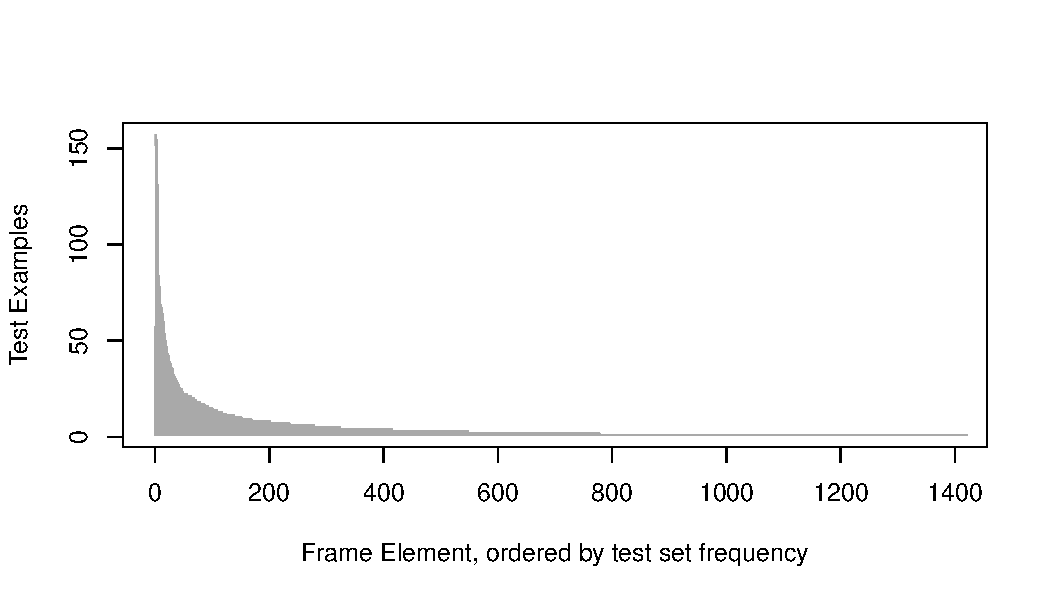
\includegraphics[width=\textwidth]{fig/num_instances}
	\end{subfigure}
	\begin{subfigure}[b]{0.5\textwidth}
		\vspace{-1cm}
		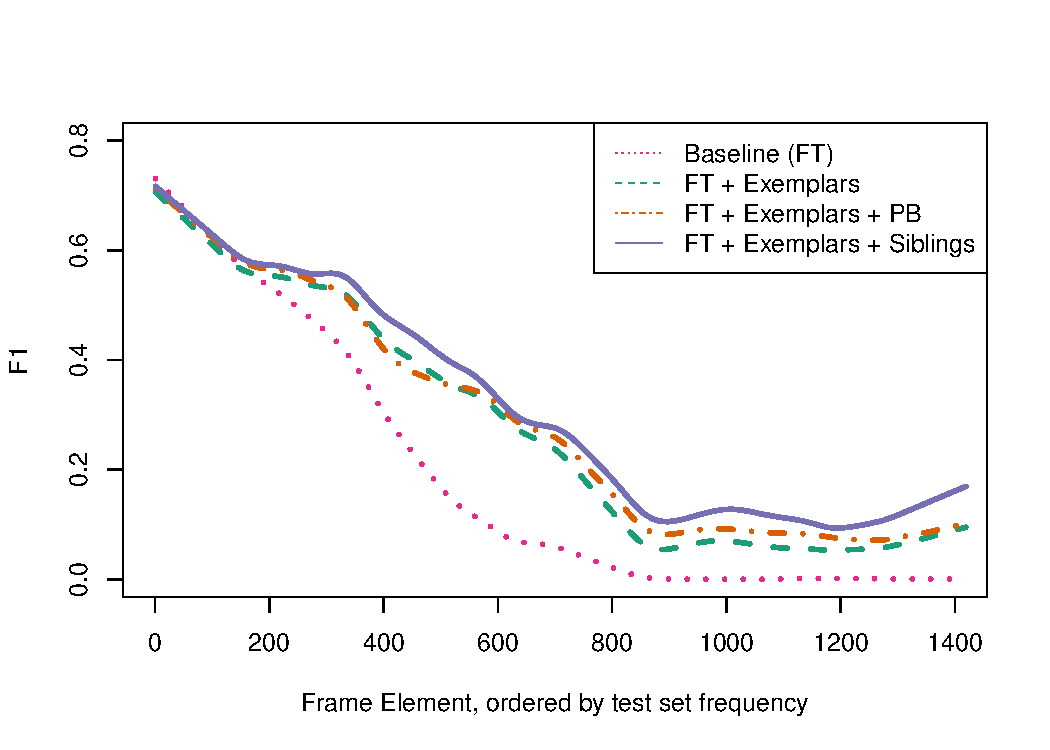
\includegraphics[width=\textwidth]{fig/f1_sorted_by_num_instances}
	\end{subfigure}
	\caption{Count and $F_1$ for each frame element appearing in the test set. $F_1$ values have been smoothed with \texttt{loess}, with a smoothing parameter of 0.2.}
\end{figure}


\section{Related Work}

\nss{Dipanjan's other papers; mention other PB SRL work?; anything using SemLink or combining resources for SRL?}

\nss{multitask learning?}

\section{Conclusion}

\nss{overall findings}

\nss{future work: testing ground for improvements to PB and SemLink; automatic mappings between resources}

\finalversion{\section*{Acknowledgments}

FUNDING}

\smaller

\bibliographystyle{style/aclnat}
% you bib file should really go here
\setlength{\bibsep}{1pt}
{\fontsize{10}{12.25}\selectfont
\bibliography{argid}}

\end{document}
